\documentclass[10pt,a4paper,openany]{book}
\usepackage[spanish]{babel}
\usepackage[version=3]{mhchem} % Package for chemical equation typesetting
\usepackage{siunitx} % Provides the \SI{}{} and \si{} command for typesetting SI units
\usepackage{graphicx} % Required for the inclusion of images
\usepackage{natbib} % Required to change bibliography style to APA
\usepackage{amsmath} % Required for some math elements 
\usepackage[left=2.54cm,right=2.54cm,top=2.54cm,bottom=2.54cm]{geometry}
\setlength\parindent{0pt} % Removes all indentation from paragraphs
\graphicspath{{./img/}}
%\renewcommand{\labelenumi}{\alph{enumi}.} % Make numbering in the enumerate environment by letter rather 
%----------------------------------------------------------------------------------------
%	DOCUMENT HEADER
%----------------------------------------------------------------------------------------
\def\BibTeX{{\rm B\kern-.05em{\sc i\kern-.025em b}\kern-.08em
    T\kern-.1667em\lower.7ex\hbox{E}\kern-.125emX}}
	\graphicspath{{./img/}}
	\usepackage{fancyhdr} % Headers and footers
	\pagestyle{fancy} % All pages have headers and footers
	\fancyhead[L]{Fac. de Ingenier\'ia y Ciencia}
	\fancyhead[C]{2020 - 2} % Custom header text
	%\fancyfoot[RO,LE]{\thepage} % Custom footer text
	\fancyhead[R]{
\includegraphics[width=0.14\linewidth]{Logo-PUJ-Negro}\vspace{-0.2cm}}
	\fancypagestyle{firstpage}{%
	\fancyhead[L]{Fac. de Ingenier\'ia y Ciencia}
	\fancyhead[C]{} % Custom header text
	\fancyhead[R]{
\includegraphics[width=0.14\linewidth]{Logo-PUJ-Negro}\vspace{-0.2cm}}
}
%----------------------------------------------------------------------------------------
%	DOCUMENT
%----------------------------------------------------------------------------------------
\begin{document}
\begin{titlepage}
	\begin{center}
		\vspace{2cm}
		{\Large \textbf{LÍNEAS DE PRODUCTOS DE SOFTWARE}}\\
		\vspace{3cm}
		{\Large \textbf{LÍNEA TALLERES VIRTUALES}}\\
		\vspace{3cm}
		{\large \today}\\
		\vspace{3cm}
		{\large \textbf{Óscar Fernando calero mayor}}\\
		{\large \textbf{William Andrey Garzón Bohórquez}}\\
		{\large \textbf{Dario Leonardo Narvaez Jacome}}\\
		\vspace{1cm}
		{\large Pontificia Universidad Javeriana de Cali}\\
		{\large Facultad de Ingeniería y Ciencias}\\
		\begin{figure}[h]
			\centering
			
\includegraphics[scale=0.8]{logo}
		\end{figure}
	\end{center} 
\end{titlepage}

\tableofcontents

%----------------------------------------------------------------------------------------
%	1 Definición del alcance
%----------------------------------------------------------------------------------------
\chapter{Definición del alcance}


%----------------------------------------------------------------------------------------
%	1.1. Estudio del mercado y de factibilidad
%----------------------------------------------------------------------------------------
\section{Estudio del mercado y de factibilidad}
%----------------------------------------------------------------------------------------
%	1.2. Análisis de inversiones costos y rentabilidad
%----------------------------------------------------------------------------------------
\section{Análisis de inversiones costos y rentabilidad}

Ya que el equipo no cuenta con un musculo de inversión grande para iniciar con la línea de productos, decidimos implementar la estrategia de desarrollo incremental, con el fin de llegar a elaborar una gran cantidad de productos los valores aquí mostrados fueron obtenidos a partir de juicio de experto\\

El costo total de una LPS se descompone en costos fijos y costos variables como lo muestra la ecuación (\ref{eqn:eqn1}), donde:\\ CFlps corresponde a los costos fijos \\ CVlps corresponde a los costos variables.

\begin{equation}
C_{TotalLPS} = (CF_{LPS} + CV_{LPS})
\label{eqn:eqn1}
\end{equation}

los costos fijos de los productos a nivel operativo se pueden expresar mediante la ecuación (\ref{eqn:eqn2}), donde: \\
  CModDown son los costos de modelar el dominio \\
  CCOnfigProd corresponde a los costos de configuración de los productos\\
  CCPlatSoft se refiere a los costos del desarrollo de la plataforma \\
  CCDefComp equivale a los costos de definición \\
  CCConcepProd se trata de los costos de conseptializacion\\
\begin{equation}
CF_{ProdNivelOp} = C_{ModDown} + C_{COnfigProd} + C_{CPlatSoft} + C_{CDefComp} + C_{CConcepProd}  
\label{eqn:eqn2}
\end{equation}


La Tabla~\ref{table:t1} mustra un calculo estimado de los costos fijos (CFProdNivelOp)
 
\begin{table}[htbp]
\centering
\begin{tabular}{|c|c|c|c|p{2.5cm}|p{2.5cm}|} \hline
 Dato & Valor(\$)/h & Esfuerzo[LPS] (h) & Total(\$)[LPS] & Esfuerzo [Tradicional] (h) & Total(\$) [Tradicional]\\[0.5ex] \hline
 CModDom     & 20000 & 40  & 800000   & 0   & 0 \\[0.5ex] \hline
 CConfigProd & 25000 & 80  & 2000000  & 50  & 1250000 \\[0.5ex] \hline
 CPlatSoft   & 30000 & 384 & 11520000 & 300 & 9000000 \\[0.5ex] \hline
 CDefComp    & 20000 & 32  & 640000   & 16  & 320000  \\[0.5ex] \hline
 CConcepProd & 18000 & 40  & 720000   & 0   & 0       \\[0.5ex] \hline
 TOTAL &  &  & 15680000 & & 10570000\\[0.5ex] \hline
\end{tabular}
\caption{Costos Fijos}
\label{table:t1}
\end{table}

En la ecuación (\ref{eqn:eqn3}) CVLPS, corresponde al costo variable de la LPS. Este costo corresponde a los costos variables de los productos de nivel operativo.

\begin{equation}
CV_{LPS} = CV_{ProdNivelOp}  
\label{eqn:eqn3}
\end{equation}

\begin{equation}
CV_{ProdNivelOp} =  C_{DerivProd} 
\label{eqn:eqn4}
\end{equation}

\begin{equation}
C_{DerivProd} = C_{ConsepPro}  +  C_{UtilizaionComp}
\label{eqn:eqn5}
\end{equation}

Los costos de conceptualización de los productos CConcepProd constituyen los costos fijos de la derivación de productos, y en tanto que costos fijos, ya fueron incluídos en los costos fijos de los productos del nivel operativo por tanto la ecuación (\ref{eqn:eqn3})  se convierte en:

\begin{equation}
CV_{LPS} = C_{UtilizaionComp} 
\label{eqn:eqn6}
\end{equation}

Los costos de utilización de los componentes en la ecuación (\ref{eqn:eqn6}) están dados por la ecuación (\ref{eqn:eqn7}) donde:\\
NpNo es el número total de productos de nivel operativo de la LPS.\\
NCompProdNop es el número total de componentes del producto p de nivel operativo.\\
CConstruccionComp j,p son los costos de construcción (costos variables) del componente j, utilizado en el producto p.\\
NumProdUsanCompj es el número de productos de nivel operativo que utilizan el componente j.\\

\begin{equation}
C_{UtilizaionComp} = \sum_{p=1}NpNo \sum_{j=1}N_{CompProdNOp}\left(\frac{C_{ContruccionComp}}{NumProdUsanComp}\right)
\label{eqn:eqn7}
\end{equation}

\begin{quote}Para determinar los costos de la utilización de componentes, los expertos estiman el grado de utilización esperado para cada componente utilizable en los productos de nivel operativo, luego dividen los costos de construcción de cada componente por su grado de utilización.\cite{8048908}, para este caso o veremos los calculos en la Tabla~\ref{table:t2}.\end{quote}


\begin{table}[htbp]
\centering
\begin{tabular}{|c|c|c|} \hline
 Dato & Producto 1  & Producto 2 \\[0.5ex] \hline
 NCompProdNop      &  12 & 16  \\[0.5ex] \hline
 CConstruccionComp &  0  & 3840000  \\[0.5ex] \hline
 NumProdUsanCompj  &  1  & 2 \\[0.5ex] \hline
 CVProdNivelOp     &  0  &  1920000 \\[0.5ex] \hline
\end{tabular}
\caption{Costos Variables}
\label{table:t2}
\end{table}

Ahora calcularemos nuestro ROI punto de equilibro para estimar cuantos productos tenemos que vender para obtener el retorno de la inversion.

\begin{table}[htbp]
\centering
\begin{tabular}{|c|c|c|c|c|c|} \hline
 Caso & Producto 1  & Producto 2 & Producto 3 & Producto 4 & Producto 5\\[0.5ex] \hline
 Sin reutilizacion  & 10570000 & 21140000 & 42280000  & 84560000  & 169120000 \\[0.5ex] \hline
 Usando LPS         & 15680000 & 17600000 & 19520000  & 21440000  & 23360000 \\[0.5ex] \hline
 Ahorro con LPS     & 5110000  & 3540000  & 22760000  & 63120000  & 145760000 \\[0.5ex] \hline
 ROI                & -0,18    & 0.13     &  0,82     & 2,28      & 5,27 \\[0.5ex] \hline
 
\end{tabular}
\caption{Calculo del ROI}
\label{table:t3}
\end{table}


La Figura~\ref{fig:grf1} muestra los datos obtenido en la Tabla~\ref{table:t3} que compara los costos para desarrollar n productos de nivel operativo bajo enfoque tradicional versus LPS

\vspace{9cm}

\begin{figure}[h]
	\centering
	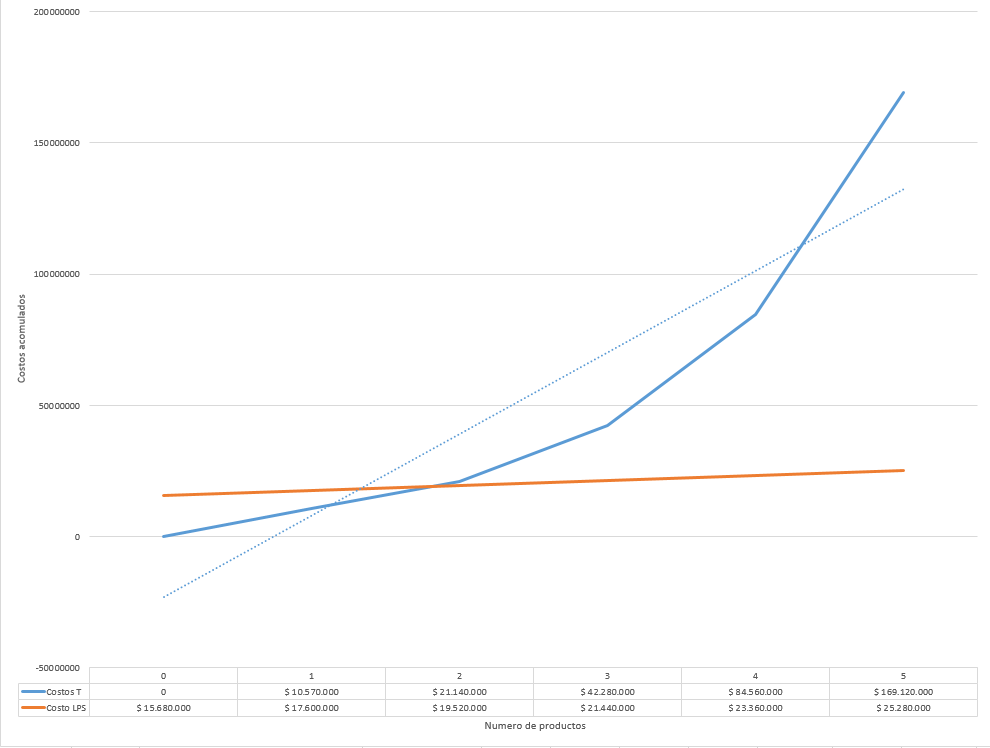
\includegraphics[width=1\textwidth]{grf1}
	\caption{Costos, enfoque tradicional versus LPS}
	\label{fig:grf1}
\end{figure} 

En conclusión, podemos ver que la rentabilidad de la línea de productos nos ofrece una rentabilidad positiva a partir del segundo producto vendido ya que la inversión inicial es de 15’680.000 COP y esta es recuperada con la venta del segundo producto, el cual se estima tiene unos costos variables de 1’920.000 COP y se vende a 17’600.000 COP produciendo una ganancia de 15’680.000 COP. 


%----------------------------------------------------------------------------------------
%	1.3. Análisis interno
%----------------------------------------------------------------------------------------
\section{Análisis interno}

\begin{table}[htbp]
\centering
\begin{tabular}{|c|p{8cm}|p{4cm}|} \hline
 Nombre & Habilildades  & Área de Conocimiento \\[0.5ex] \hline
 Oscar & PHP, Angular   & Automotriz, Financiero \\[0.5ex] \hline
 William & Java, Angular, Python, JavaScript ,Spring MVC, BOOT, SECURITY, JSP, HTML, CSS, BOOTSTRAP, Thymeleaf, Hibernatem, SQL, WebService REST, SOAP   & Financiero, Bancario \\[0.5ex] \hline
 Dario & Java/Groovy, Angular   & Expedición Documentos Civiles, Domicilios \\[0.5ex] \hline
\end{tabular}
\caption{Análisis interno}
\label{table:t4}
\end{table}

\vspace{9cm}
%----------------------------------------------------------------------------------------
%	1.4. Definición del catálogo del producto
%----------------------------------------------------------------------------------------
\section{Definición del catálogo del producto}


\begin{table}[htbp]
\centering
\begin{tabular}{|p{5cm}|p{3cm}|p{3cm}|p{3cm}|} \hline
	& \textbf{Básico}  
	\begin{itemize}
		\item Mecánica
		\item Lavado
	\end{itemize} 
	& \textbf{Profesional} 
	\begin{itemize}
		\item Mecánica
		\item Lavado
		\item Pintura
	\end{itemize} 
	& \textbf{Experto}
	\begin{itemize}
		\item Mecánica
		\item Lavado
		\item Pintura
		\item Audio
	\end{itemize}  \\[0.5ex] \hline
Ingreso Anual$<$ \$1.131.000.000	                & TallerVirtual1  &  &  \\[0.5ex] \hline
\$1.131.000.000$<$ Ingreso Anual$<$ \$4.523.000.000	&   & TallerVirtual2 &  \\[0.5ex] \hline
Ingreso Anual $>$ \$4.523.000.000	                &   &  & TallerVirtual3 \\[0.5ex] \hline

\end{tabular}
\caption{Tabla de Segmentos 1}
\label{table:t5}
\end{table}


\begin{table}[htbp]
\centering
\begin{tabular}{|p{5cm}|p{3cm}|p{3cm}|p{3cm}|} \hline
	& \textbf{Básico}  
	\begin{itemize}
		\item Reserva
	\end{itemize} 
	& \textbf{Profesional} 
	\begin{itemize}
		\item Reserva
		\item Selección de servicios
	\end{itemize} 
	& \textbf{Experto}
	\begin{itemize}
		\item Reserva
		\item Selección de servicios
		\item Selección de mecánico
	\end{itemize}  \\[0.5ex] \hline
Ingreso Anual$<$ \$1.131.000.000	                & TallerVirtual1  &  &  \\[0.5ex] \hline
\$1.131.000.000$<$ Ingreso Anual$<$ \$4.523.000.000	&   & TallerVirtual2 &  \\[0.5ex] \hline
Ingreso Anual $>$ \$4.523.000.000	                &   &  & TallerVirtual3 \\[0.5ex] \hline

\end{tabular}
\caption{Tabla de funcionalidades}
\label{table:t6}
\end{table}


¿Quiénes son los principales actores de la industria?
\begin{itemize}
	\item Montallantas
	\item Lavado de autos
	\item Talleres Automotrices
	\item Pintura Automotriz
\end{itemize} 

¿Hacia dónde están visionando sus objetivos?
\begin{itemize}
	\item Creación de 3  productos ajustados de acuerdo al nivel de especialidad del taller automotriz
\end{itemize} 

¿Vale la pena la inversión en este segmento?
\begin{itemize}
	\item Permite generar una estructuración personalizada de los servicios ofrecidos para cada taller
\end{itemize}

¿Hemos descubierto un nuevo nicho de mercado?
\begin{itemize}
	\item No, pero se permitiría la flexibilidad de incorporar o eliminar servicios ofrecidos por el taller
\end{itemize}

%----------------------------------------------------------------------------------------
%	1.4.1. Catálogo de Productos
%----------------------------------------------------------------------------------------
\subsection{Catálogo de Productos}

\begin{enumerate}
	\item TallerVirtual1:
	\begin{itemize}
		\item Reserva de atención (sin pago)
		\item Lista de servicios (no se pueden seleccionar, se agregan por BD)
	\end{itemize}
	\item TallerVirtual2:
	\begin{itemize}
		\item Reserva de atención (con pago dependiendo de los servicios seleccionados)
		\item Lista de servicios (se pueden seleccionar, ingresados por excel)
	\end{itemize}
	\item TallerVirtual3:
	\begin{itemize}
		\item Reserva de atención (con pago, dependiendo de los servicios seleccionados y mecánico)
		\item Lista de servicios (se pueden seleccionar, ingresados por backend)
		\item Lista de mecánicos(se pueden seleccionar, ingresados por backend)
	\end{itemize}
\end{enumerate}




%----------------------------------------------------------------------------------------
%	1.5 Evolución
%----------------------------------------------------------------------------------------
\section{Evolución}






\medskip
\bibliographystyle{abbrv}
\bibliography{libreria}

\end{document}
